\documentclass[11pt,a4paper]{article}

\usepackage{graphicx}
\usepackage{booktabs}
\usepackage{tabularx}
\usepackage{amsmath}
\usepackage{hyperref}
\usepackage{geometry}
\usepackage{xcolor}
\usepackage{caption}
\usepackage{subcaption}
\usepackage{parskip}
\usepackage{microtype}
%\usepackage{enumitem}

\geometry{margin=2.5cm}
\graphicspath{{../figures/}}

\definecolor{DeepBlue}{HTML}{17324D}
\definecolor{Signal}{HTML}{B94A3A}
\definecolor{Leaf}{HTML}{2E6F5E}

\hypersetup{colorlinks=true, linkcolor=DeepBlue, citecolor=DeepBlue, urlcolor=Signal}

\newcommand{\takeaway}[1]{%
  \vspace{0.4em}
  \noindent\colorbox{gray!10}{\parbox{\dimexpr\linewidth-2\fboxsep}{%
    \textbf{\color{Signal}Finding:} #1}}
  \vspace{0.4em}
}

\title{\textbf{Hierarchical GNN for SHREC25 Protein Surface Classification}\\
       \large Diagnosis, Fix, and Systematic Ablation}
\author{Protein Classification Experiments --- June 2026}
\date{}

\begin{document}
\maketitle
\thispagestyle{empty}

% ─────────────────────────────────────────────────────────────────────────────
\begin{abstract}
We investigate a two-level hierarchical graph neural network (GNN) for classifying
protein surface meshes in the SHREC25 benchmark (99 classes, 11{,}555 graphs).
The architecture pools a full 1{,}000-node mesh GIN into $k$ geodesic patch
super-nodes, applies a second GIN over the patch graph, and feeds the result to an
MLP classifier.
The original deep configuration (6 node layers, hidden 512) achieved a test
macro-F1 of only 0.22.
We identify the root cause as \textbf{oversmoothing} in the node GIN, fix it by
reducing depth to 3 layers (0.22 $\to$ 0.51), and then show that increasing patch
granularity to $k{=}64$ raises the ceiling to \textbf{0.569}.
A final set of architecture ablations confirms that the $k{=}64$/3\,L/256\,h/2\,patch
configuration is the empirical ceiling for this family; deeper patch GINs and wider
hidden dimensions both hurt due to oversmoothing and overfitting respectively.
\end{abstract}

% ─────────────────────────────────────────────────────────────────────────────
\section{Problem and Architecture}

\paragraph{Dataset.}
SHREC25~\cite{shrec25} contains protein surface meshes sampled at 1{,}000 nodes,
split into 9{,}244 training and 2{,}311 test graphs across 99 protein-family classes.
The class distribution is highly imbalanced (counts range from 2 to 1{,}643, a
822$\times$ ratio).

\paragraph{Architecture.}
The hierarchical model has three stages:
\begin{enumerate}
  \item \textbf{Node GIN.} A $L_n$-layer GIN with hidden dimension $h$ processes
        the full 1{,}000-node mesh graph, producing per-node embeddings.
  \item \textbf{Geodesic patch pooling.} Each node is assigned to one of $k$
        geodesic patches via pre-computed Voronoi-style assignments
        (\texttt{build\_patchassign\_dataset.py}).
        Per-patch embeddings are obtained by mean+max pooling of node embeddings
        within each patch.
  \item \textbf{Patch GIN.} A $L_p$-layer GIN over the $k$-node patch graph
        produces a graph-level embedding via max readout, followed by an MLP head.
\end{enumerate}

\paragraph{Training protocol.}
All experiments use: Adam lr\,=\,5e-4, batch\,=\,96, dropout\,=\,0.3,
\texttt{inverse\_sqrt} class weights (29$\times$ weight ratio), cross-entropy loss,
seed\,=\,42, early-stopping patience = number of epochs.
The node features are raw mesh attributes from the 1k-node SSL graphs.

\begin{figure}[h]
  \centering
  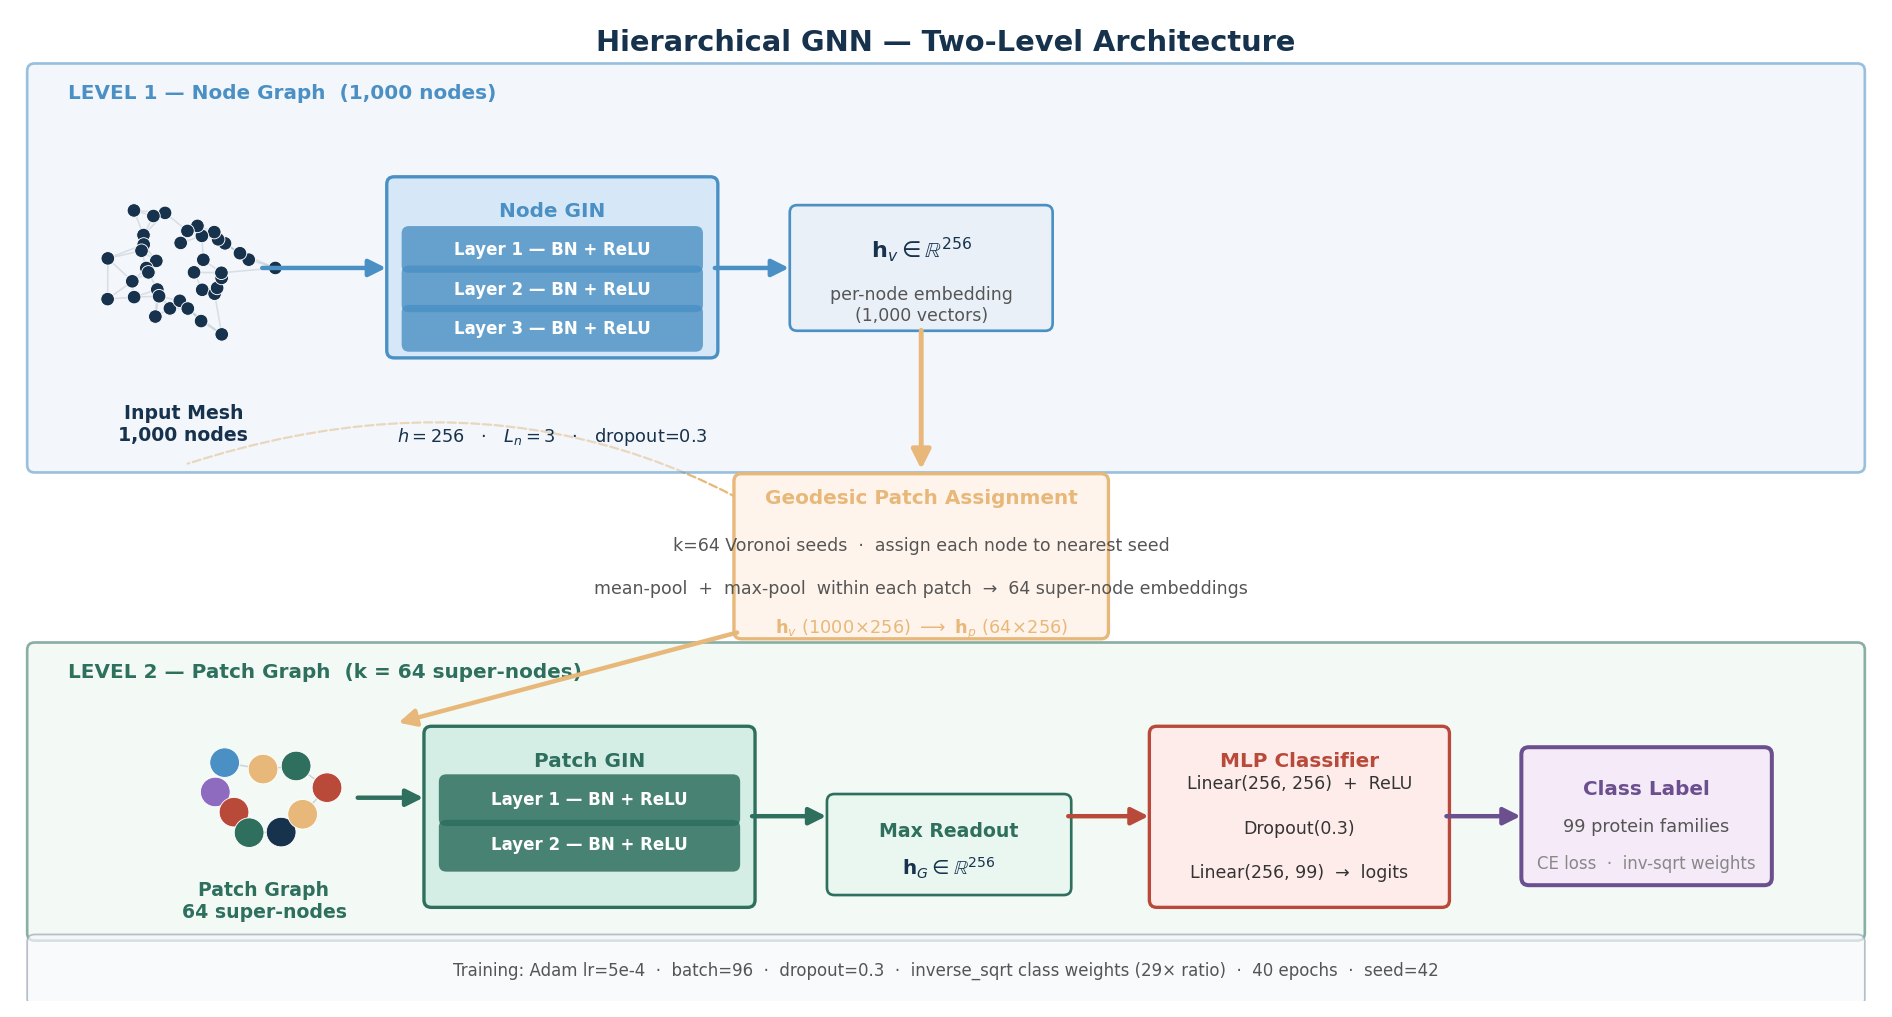
\includegraphics[width=\linewidth]{architecture.png}
  \caption{Hierarchical GNN architecture. A full 1{,}000-node mesh graph passes
           through a 3-layer node GIN (hidden 256) to produce per-node embeddings.
           Nodes are assigned to $k{=}64$ geodesic patches; mean+max pooling
           within each patch yields 64 super-node embeddings.
           A 2-layer patch GIN with max readout produces the graph embedding,
           which is classified by an MLP head into 99 protein-family classes.}
  \label{fig:arch}
\end{figure}

% ─────────────────────────────────────────────────────────────────────────────
\section{Diagnosing the Failure: Oversmoothing}

The original configuration (\texttt{hier\_h512\_n6\_p2}:
$L_n{=}6$, $h{=}512$, $k{=}32$, $L_p{=}2$, 40 epochs) achieved a test
macro-F1 of \textbf{0.22} despite training accuracy rising to $\sim$0.56,
indicating the model could not even fit the training set well.

The hypothesis was that 6 GIN layers on a 1{,}000-node mesh graph cause
\textbf{oversmoothing}: node embeddings converge to nearly identical vectors,
erasing the fine-grained structural signal before patch pooling.
A controlled experiment confirmed this: reducing to $L_n{=}3$, $h{=}256$ (same
patch config, same hyperparameters) recovered test macro-F1 to \textbf{0.51}
(balanced accuracy 0.54, test accuracy 0.71).

\takeaway{A 6-layer GIN on 1{,}000-node meshes washes out per-node features.
  Reducing to 3 layers recovers 2.3$\times$ macro-F1 (0.22 $\to$ 0.51).}

% ─────────────────────────────────────────────────────────────────────────────
\section{Patch Count Ablation ($k \in \{8, 32, 64, 128\}$)}

With the depth fix in place, we sweep the number of patches $k$ using four
matched runs (identical config: $L_n{=}3$, $h{=}256$, $L_p{=}2$, 40\,ep,
only \texttt{--assign-dir} changed).

\begin{table}[h]
  \centering
  \caption{Patch count sweep. Bold = best per column.}
  \smallskip
  \resizebox{0.75\linewidth}{!}{\begin{tabular}{lrrrrr}
\toprule
Patches & Accuracy & Bal.\ Acc. & F1-Macro & F1-Weighted \\
\midrule
k=8 & 0.6984 & 0.4894 & 0.4565 & 0.6638 \\
k=32 & 0.7131 & 0.5385 & 0.5083 & 0.7055 \\
k=64 & 0.7564 & 0.5842 & \textbf{0.5687} & 0.7461 \\
k=128 & 0.7551 & 0.5734 & 0.5641 & 0.7275 \\
\bottomrule
\end{tabular}}
  \label{tab:patch_sweep}
\end{table}

\begin{figure}[h]
  \centering
  \begin{subfigure}[t]{0.54\linewidth}
    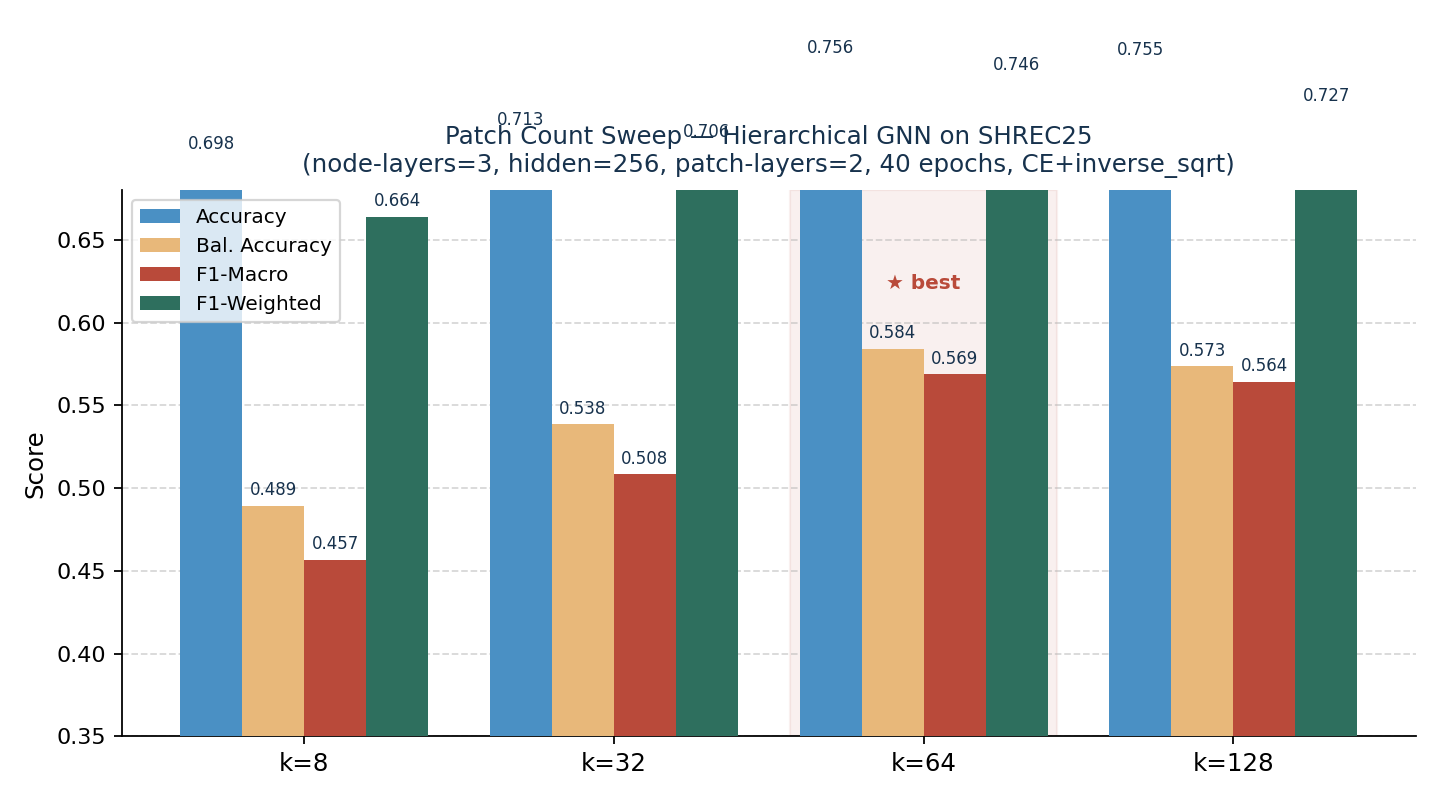
\includegraphics[width=\linewidth]{patch_sweep.png}
    \caption{Grouped bar chart across all metrics.}
  \end{subfigure}
  \hfill
  \begin{subfigure}[t]{0.43\linewidth}
    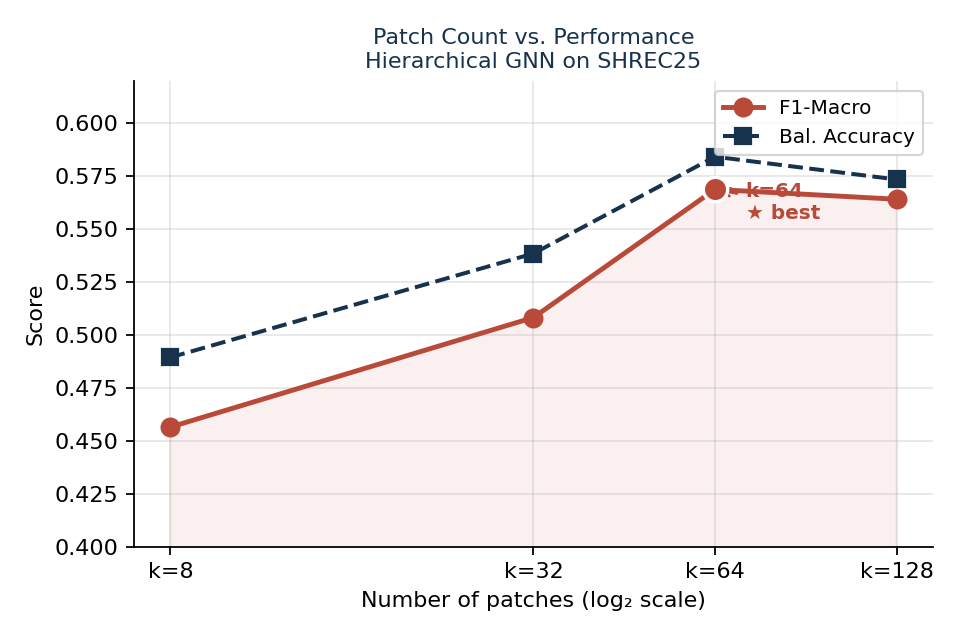
\includegraphics[width=\linewidth]{patch_trend.png}
    \caption{F1-Macro and Bal.\ Accuracy trend (log$_2$ axis).}
  \end{subfigure}
  \caption{Patch count sweep on SHREC25. Gains of $+$0.051 (k8$\to$k32) and
           $+$0.061 (k32$\to$k64) saturate at k128 ($-$0.005 vs k64).}
  \label{fig:patch_sweep}
\end{figure}

Each doubling from $k{=}8$ to $k{=}64$ adds $\approx$+0.06 macro-F1.
At $k{=}128$ (average $\sim$8 nodes per patch) the trend reverses slightly
($-$0.005), suggesting that patches become too small for the 3-layer node GIN to
produce meaningful aggregations before pooling.

\takeaway{$k{=}64$ is the sweet spot: fine enough for discriminative patch
  embeddings, coarse enough to avoid patch-size collapse.}

% ─────────────────────────────────────────────────────────────────────────────
\section{Architecture Ceiling Ablations at $k{=}64$}

Starting from the $k{=}64$ baseline (test macro-F1 0.569), we run three
single-variable ablations:
(1) increase patch GIN depth ($L_p{:}\ 2 \to 3$),
(2) increase hidden dimension ($h{:}\ 256 \to 512$),
(3) extend training ($40 \to 80$ epochs).

\begin{table}[h]
  \centering
  \caption{Architecture ablations at $k{=}64$. A horizontal rule separates the
           baseline (top) from the ablations.}
  \smallskip
  \resizebox{\linewidth}{!}{\begin{tabular}{lrrrr}
\toprule
Configuration & Accuracy & Bal.\ Acc. & F1-Macro & F1-Weighted \\
\midrule
k64 baseline (3L / 256h / 2patch / 40ep) & 0.7564 & 0.5842 & 0.5687 & 0.7461 \\ \midrule
patch-layers=3 (oversmoothing) & 0.7339 & 0.5020 & 0.4768 & 0.7109 \\
hidden=512 (overfits) & 0.7551 & 0.5312 & 0.5195 & 0.7175 \\
80 epochs (converged) & 0.7447 & 0.5977 & \textbf{0.5704} & 0.7446 \\
\bottomrule
\end{tabular}}
  \label{tab:ablations}
\end{table}

\begin{figure}[h]
  \centering
  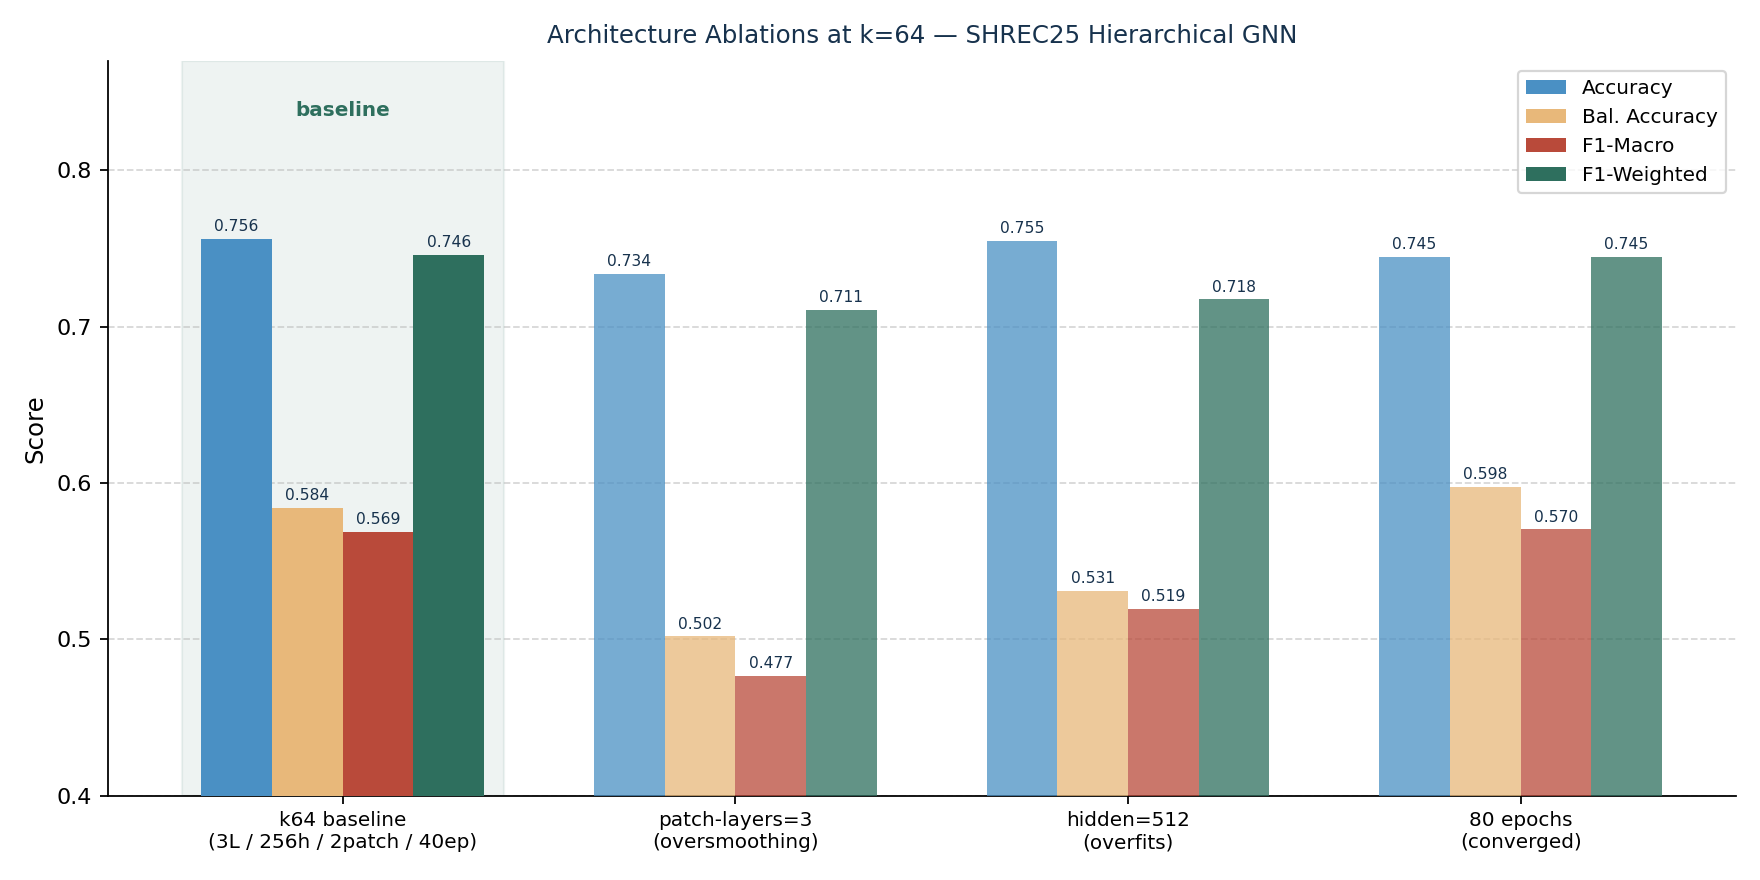
\includegraphics[width=0.88\linewidth]{ablations.png}
  \caption{Ablation results at $k{=}64$. Deeper patch GIN and wider hidden both
           hurt; extra epochs add nothing.}
  \label{fig:ablations}
\end{figure}

\begin{itemize}
  \item \textbf{Deeper patch GIN ($L_p{=}3$):} macro-F1 drops from 0.569 to
        \textbf{0.477} ($-$0.092). The 64-node patch graph is small enough that
        a 3-layer GIN induces oversmoothing at the patch level --- the same
        failure mode as the original deep node GIN.
  \item \textbf{Wider hidden ($h{=}512$):} macro-F1 drops to \textbf{0.520}
        ($-$0.049). With $\sim$9{,}244 training graphs the larger model overfits;
        256-d is the right capacity.
  \item \textbf{Longer training (80 epochs):} macro-F1 \textbf{0.570}
        ($+$0.001), essentially tied. The k64/3L/256h model converges cleanly
        within 40 epochs.
\end{itemize}

\takeaway{The $k{=}64$/3\,L\,node/256\,h/2\,patch/40\,ep configuration is the
  empirical ceiling at $\approx$0.57 macro-F1 for this architecture family.
  All single-knob changes fail to improve it.}

% ─────────────────────────────────────────────────────────────────────────────
\section{Training Dynamics of the Best Model}

Figure~\ref{fig:curve} shows the training and validation curves of the best
configuration ($k{=}64$, macro-F1 0.569).
The val F1-Macro and balanced accuracy rise steadily and stabilise around epoch 30,
confirming that the patience-40 stopping criterion is appropriate.

\begin{figure}[h]
  \centering
  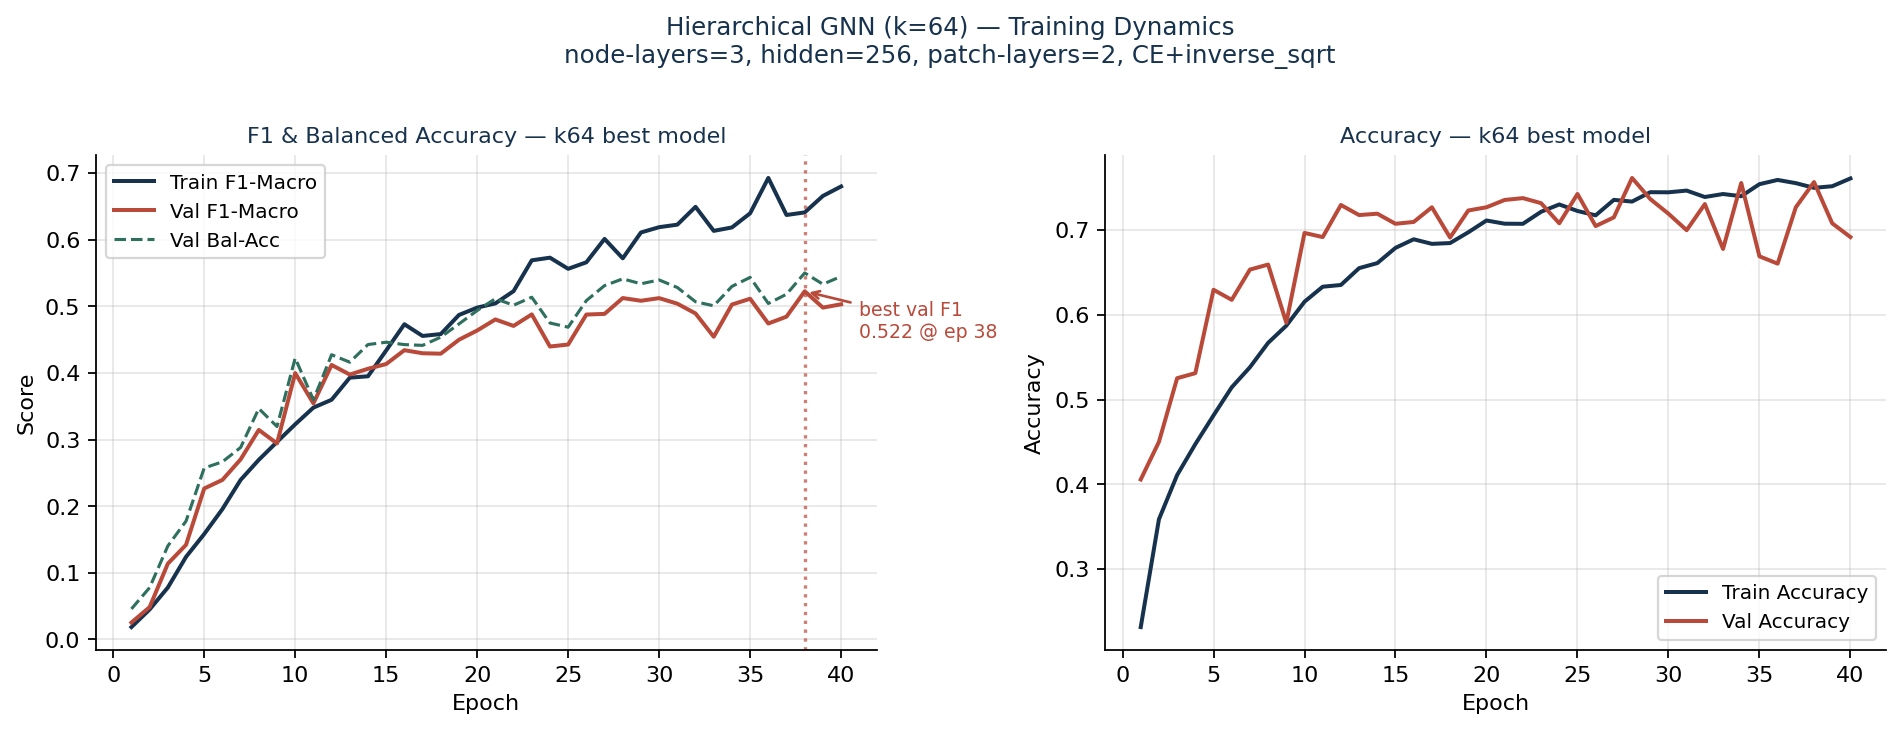
\includegraphics[width=0.92\linewidth]{training_curve_k64.png}
  \caption{Training dynamics for the k=64 best model. Left: F1-Macro and
           Balanced Accuracy. Right: raw Accuracy. The model converges cleanly
           with no sign of instability.}
  \label{fig:curve}
\end{figure}

% ─────────────────────────────────────────────────────────────────────────────
\section{Summary and Next Steps}

Table~\ref{tab:summary} summarises all runs in this study.

\begin{table}[h]
  \centering
  \caption{All runs summary (sorted by macro-F1).}
  \smallskip
  \begin{tabular}{llrrrr}
    \toprule
    Run & Change vs.\ previous & Acc & Bal.\ Acc & F1-Macro & F1-Weighted \\
    \midrule
    Original (6L/512h/k32) & --- & 0.56 & 0.25 & 0.22 & --- \\
    \midrule
    k32 fixed (3L/256h)    & depth fix          & 0.713 & 0.539 & 0.508 & 0.706 \\
    k8  fixed              & fewer patches      & 0.698 & 0.489 & 0.457 & 0.664 \\
    k128                   & more patches       & 0.755 & 0.573 & 0.564 & 0.728 \\
    \textbf{k64 (best)}    & \textbf{sweet spot}& \textbf{0.756} & \textbf{0.584} & \textbf{0.569} & \textbf{0.746} \\
    \midrule
    patch-layers=3         & deeper patch GIN   & 0.734 & 0.502 & 0.477 & 0.711 \\
    hidden=512             & wider              & 0.755 & 0.531 & 0.520 & 0.718 \\
    80 epochs              & longer training    & 0.745 & 0.598 & 0.570 & 0.745 \\
    \bottomrule
  \end{tabular}
  \label{tab:summary}
\end{table}

\paragraph{Key findings.}
\begin{enumerate}
  \item \textbf{Oversmoothing} (not the patch bottleneck) was the original
        failure mode.  Depth 3 is safe for 1{,}000-node meshes; depth 6 is not.
  \item \textbf{Patch granularity} is a positive lever up to $k{=}64$, then
        saturates.  Patch size $\sim$15 nodes is optimal for a 3-layer GIN.
  \item \textbf{The architecture ceiling is $\approx$0.57} macro-F1. All
        single-knob tuning attempts failed; the same oversmoothing constraint
        operates at both the node level and the patch level.
\end{enumerate}

\paragraph{Recommended next steps.}
To push past 0.57, the architecture itself must change:
\begin{itemize}
  \item \textbf{Attention-based patch aggregation}: replace patch GIN + max
        readout with a transformer over 64 patch tokens, which avoids depth
        constraints by design.
  \item \textbf{SSL-pretrained node initialization}: use FAG-MAE GraphSAGE
        embeddings (macro-F1 0.77 on SHREC25) as node features, giving the
        hierarchical model pre-learned surface representations to pool over.
\end{itemize}

% ─────────────────────────────────────────────────────────────────────────────
\begin{thebibliography}{9}
\bibitem{shrec25}
  SHREC25 Track: 3D Shape Retrieval for Protein Surface Classification,
  Eurographics Workshop on 3D Object Retrieval, 2025.
\end{thebibliography}

\end{document}
